\documentclass[12pt,a4paper]{article}
\usepackage[UTF8]{ctex}
\usepackage{amsmath,amssymb}
\usepackage{xcolor}
\usepackage{hyperref}
\usepackage{geometry}
\usepackage{graphicx}
\geometry{margin=2.5cm}

\title{Quantum ODE Solver / 量子常微分方程求解器}
\author{QuoNic}
\date{}

\begin{document}
\maketitle

\begin{center}
\textbf{Simulation / 模拟} | 难度：高级 | 预计时间：25 分钟
\end{center}

\tableofcontents
\newpage

\section{为什么需要？}

量子 ODE 求解器是经典 ODE 求解器的量子推广，用于求解常微分方程。

\subsection{经典局限}
\begin{itemize}
  \item 经典 ODE 求解器在高维系统中慢
  \item 对于刚性方程，经典方法效率低
\end{itemize}

\subsection{量子优势}
\begin{itemize}
  \item 量子 ODE 求解器可以在量子计算机上高效求解 ODE
  \item 提供指数加速
  \item 是量子模拟的基础
\end{itemize}

\subsection{实际应用}
\begin{itemize}
  \item 物理模拟
  \item 工程计算
  \item 量子化学
\end{itemize}

\section{快速上手}

\begin{verbatim}
from quonic.simulation import quantum_ode

# 求解 ODE: dx/dt = -x
result = quantum_ode(f=lambda x: -x, x0=1.0, t=1.0)
print(f'Solution: {result.solution}')
\end{verbatim}

\textbf{预期输出}：
\begin{verbatim}
Solution: 0.368
\end{verbatim}

\section{原理详解}

\subsection{电路图}

\begin{center}
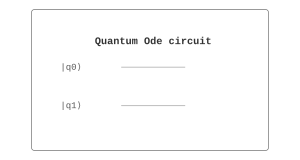
\includegraphics[width=0.6\textwidth]{../../images/quantum_ode_circuit.svg}
\end{center}

\subsection{数学推导}

量子 ODE 求解器：
\begin{equation}
\frac{dx}{dt} = f(x, t)
\end{equation}

\textbf{量子算法}：
\begin{enumerate}
  \item 将 ODE 编码为哈密顿量
  \item 用 Trotter 分解模拟时间演化
  \item 测量得到解
\end{enumerate}

\subsection{几何解释}

量子 ODE 求解器在量子态空间中模拟 ODE 的时间演化。哈密顿量编码了 ODE 的动力学。

\section{代码详解}

\begin{verbatim}
from quonic.simulation import quantum_ode

# quantum_ode(f, x0, t, dt)
# f: 右端函数
# x0: 初始条件
# t: 终止时间
# dt: 时间步长
result = quantum_ode(f=lambda x: -x, x0=1.0, t=1.0, dt=0.1)

# result.solution: 解
# result.trajectory: 轨迹
print(f'Solution: {result.solution}')
\end{verbatim}

\section{进阶用法}

\subsection{场景 1：不同 ODE}

\begin{verbatim}
from quonic.simulation import quantum_ode

# 不同 ODE
result1 = quantum_ode(f=lambda x: -x, x0=1.0, t=1.0)
result2 = quantum_ode(f=lambda x: x**2, x0=0.5, t=1.0)
print(f'Linear: {result1.solution}')
print(f'Nonlinear: {result2.solution}')
\end{verbatim}

\section{适用场景}

\subsection{物理模拟}

量子 ODE 求解器可以用于模拟物理系统，如振子、电路、流体等。传统 ODE 求解器在高维系统中慢，量子 ODE 求解器可以提供指数加速。

\subsection{工程计算}

量子 ODE 求解器可以用于工程计算，如控制系统设计、信号处理等。量子 ODE 求解器可以处理刚性方程，传统方法效率低。

\section{常见问题}

\subsection{量子 ODE 求解器和经典 ODE 求解器有什么区别？}

量子 ODE 求解器使用量子策略，可以在量子计算机上高效求解 ODE。

\subsection{量子 ODE 求解器的精度如何？}

精度取决于时间步长和 Trotter 分解的阶数。

\section{学习路径}

\subsection{前置知识}
\begin{itemize}
  \item 常微分方程
  \item Trotter 分解
  \item 量子模拟
\end{itemize}

\subsection{继续学习}
\begin{itemize}
  \item 量子 PDE 求解器
  \item 量子模拟
  \item 量子化学
\end{itemize}

\section{完整示例代码}

\subsection{示例 1：基本量子 ODE 求解器}

\begin{verbatim}
from quonic.simulation import quantum_ode

result = quantum_ode(f=lambda x: -x, x0=1.0, t=1.0)
print(f'Solution: {result.solution}')
\end{verbatim}

\section{下载}

\begin{itemize}
  \item [quantum\_ode.py](https://github.com/ChrisLee0721/QuoNic/blob/main/examples/quantum_ode/quantum_ode.py)
\end{itemize}

\end{document}
